\chapter{Lec15 20220325}

Topics

\begin{enumerate}
    \item What's so hard about interaction?
    \item Bare electron propagator
    \item Full electron propagator
\end{enumerate}

Goals

\begin{enumerate}
    \item Appreciating the steps it takes to develop perturbation theory
    \item Familiarizing with the one-particle Green's function
\end{enumerate}

\section{Interacting, so what?}

Let's first recall where we were last time. We considered an interacting problem of electrons, given schematically by
\[ \hat{H}=\hat{H}_0+\hat{V}\]
\[ \hat{H}_0\sim t\hat{c}^{\dagger}\hat{c}\]
\[ \hat{V}\sim V\hat{c}^{\dagger}\hat{c}^{\dagger}\hat{c}\hat{c}\]
and we asked what is, for instance, the dielectric function of the system. They key point to note is that
\[ \phi \left( r \right) \sim \frac{\rho _{\mathrm{ext}}}{\varepsilon r}\sim \frac{\rho _{\mathrm{tot}}}{\varepsilon _0r}\]
\[ \rho _{\mathrm{tot}}=\rho _{\mathrm{ext}}+\rho _{sc}\]
where $\rho_{\text{sc}}$ encodes how the system responds to the external potential, and in linear response is given by
\[ \delta \rho \left( t \right) \sim -\chi ^{\mathrm{ret}}\left( t \right) \rho _{\mathrm{ext}}\]
\[ \chi ^{\mathrm{ret}}\left( t \right) =i\Theta \left( t \right) \left< \left[ \hat{\rho}\left( t \right) ,\hat{\rho}\left( 0 \right) \right] \right> \]
is the retarded density-density response function of the interacting problem. (Note: we have deliberately kept the discussion schematic above, and ignored all the spatial / momentum dependence etc.)

In principle, we can go ahead and compute the expectation value. Before attempting that, however, let us make a clarification remark about the interaction pictures involved:

\begin{enumerate}
    \item Linear response: Full, interacting Hamiltonian as the unperturbed problem and the external ``probe'' as the perturbation. The susceptibility are understood to be in the Heisenberg picture with respect to the full interacting Hamiltonian
    \item Adiabatic turning on: ``Bare'', solvable (non-interacting / free / Gaussian) Hamiltonian as the unperturbed problem and ``adiabatic turning on of interactions'' as the perturbation.
\end{enumerate}

These two are really quite different. In particular, we bear in mind that the susceptibility (is equal to retarded density-density response function) is a Heisenberg picture quantity with respect to the full Hamiltonian
\[ \chi ^{\mathrm{ret}}\left( t \right) =i\Theta \left( t \right) \langle \Omega _H|\left[ \hat{\rho}_H\left( t \right) ,\hat{\rho}_H\left( 0 \right) \right] |\Omega _H\rangle \]
We also call this a retarded two-particle Green's function. ``Two-particle'' because each density operator $\hat{\rho}\sim \hat{c}^{\dagger}\hat{c}$.

Here, the ground state $|\Omega_H\rangle$ is that of the interacting problem $\hat{H}=\hat{H}_0+\hat{V}$.

Furthermore, we do not immediately know how to evaluate this expression! Recall, to take advantage of the magic of the S-matrix, time-ordering, and adiabatic turning on, we focused on the time-ordered Green's function, so the closest analog we have is
\[ \chi ^{\mathcal{T}}\left( t \right) =\langle \Omega _H|\mathcal{T} \left[ \hat{\rho}_H\left( t \right) \hat{\rho}_H\left( 0 \right) \right] |\Omega _H\rangle \]
which can now be rewritten, though the adiabatic turning on, into a formal expression
\[ \chi ^{\mathcal{T}}\left( t \right) =\frac{\langle \Omega _0|\mathcal{T} \left[ \hat{\rho}_I\left( t \right) \hat{\rho}_I\left( 0 \right) \exp \left( -i\int_{-\infty}^{\infty}{dt'\hat{V}_I\left( t' \right)} \right) \right] |\Omega _0\rangle}{\langle \Omega _0|\mathcal{T} \left[ \exp \left( -i\int_{-\infty}^{\infty}{dt'\hat{V}_I\left( t' \right)} \right) \right] |\Omega _0\rangle}\]
The numerator can be expanded in a Dyson's series
\begin{align*}
    &\langle \Omega _0|\mathcal{T} \left[ \hat{\rho}_I\left( t \right) \hat{\rho}_I\left( 0 \right) \exp \left( -i\int_{-\infty}^{\infty}{dt'\hat{V}_I\left( t' \right)} \right) \right] |\Omega _0\rangle \\
    =&\sum_{n=0}^{\infty}{\frac{\left( -i \right) ^n}{n!}\int_{-\infty}^{\infty}{dt_1dt_2\cdots dt_n\langle \Omega _0|\mathcal{T} \left[ \hat{\rho}_I\left( t \right) \hat{\rho}_I\left( 0 \right) \hat{V}_I\left( t_1 \right) \hat{V}_I\left( t_2 \right) \cdots \hat{V}_I\left( t_n \right) \right] |\Omega _0\rangle}}
\end{align*}
where the expectation value to take is, schematically,
\[ V^n\langle \Omega _0|\mathcal{T} \left[ \hat{c}_{t}^{\dagger}\hat{c}_t\hat{c}_{0}^{\dagger}\hat{c}_0\;\hat{c}_{t_1}^{\dagger}\hat{c}_{t_1}^{\dagger}\hat{c}_{t_1}\hat{c}_{t_1}\;\hat{c}_{t_2}^{\dagger}\hat{c}_{t_2}^{\dagger}\hat{c}_{t_2}\hat{c}_{t_2}\cdots \;\hat{c}_{t_n}^{\dagger}\hat{c}_{t_n}^{\dagger}\hat{c}_{t_n}\hat{c}_{t_n} \right] |\Omega _0\rangle \]
where, for sanity's sake, we have dropped all labels and instead used the subscript to denote the time. Bear in mind that, here, $t$ and $0$ are ``external'' and $t_1,t_2,\cdots,t_n$ are all integrated over.

We know how to evaluate such an expression. It's ``just'' Wick's theorem and contractions! We know that the answer will be some combinatorial product of our basic building block
\[ G_0\left( q,t \right) =\langle \Omega _0|\mathcal{T} \left[ \hat{c}_q\left( t \right) \hat{c}_{q}^{\dagger}\left( 0 \right) \right] |\Omega _0\rangle \]
known as the (bare) Feynman propagator.

A brute force evaluation for the lowest orders, say up to $V^2$, may seem perhaps tedious but possibly doable. But, it is wrong to think that such a calculation will suffice for finding the lowest order interaction corrections: we have to remember there is also a denominator, which is essentially the same power series but without the ``density-density'' part! Fortunately, as we have seen from the statistics mechanics correspondence, there is a way to handle both the numerator and the denominator in one-shot: by taking log!

In the following, we address these challenges, one at a time. Before we lose sight of the picture and get buried in the technical details, it may be good to first summarize how we will attack the problem

\begin{enumerate}
    \item Evaluate the ``bare'' (Feynman) propagator
    \item Attempt to evaluate the Dyson's series by ``brute force'', through Wick's theorem to Feynman diagrams as a mnemonic
    \item Take care of the denominator: linked cluster theorem
    \item Dyson's equation and dressed propagators: resummation of series and 1PI
    \item Partial resummation and approximations
    \item Analytic continuation and going back to real time
\end{enumerate}

\section{Bare (Feynman) propagator}

The starting point of our perturbation theory is, of course, the unperturbed problem. Here, we consider the ``free'' part of the problem, with the Hamiltonian
\[ \hat{H}_0=\sum_{x,y,\sigma ,\sigma '}{\hat{c}_{x\sigma}^{\dagger}h_{xy}^{\sigma \sigma '}\hat{c}_{y\sigma '}}\]
As discussed briefly (c.f. lecture on localized electrons), we can define ``eigenmodes'' such that
\[ \hat{H}_0=\sum_i{\varepsilon _i\hat{\tilde{c}}_{i}^{\dagger}\hat{\tilde{c}}_i}=\sum_i{\varepsilon _i\hat{\tilde{n}}_i}\]
is readily diagonalized, with all the eigenstates built by specifying the values $\hat{\tilde{n}}_i=0,1$ for the full set of mutually commuting number operators.

The ground state, i.e., the lowest energy state, is constructed by setting
\[ \tilde{n}_i=\begin{cases}
	1,\quad \mathrm{if} \varepsilon _i<0\\
	0,\quad \mathrm{if} \varepsilon _i>0\\
\end{cases}\]
and occupation of modes with exactly $\varepsilon _i=0$ does not affect the energy of the state. Such zero modes, if exist, lead to ground-state degeneracy.

Furthermore, these are eigenmodes, in the sense that their equations of motion are simply
\[ i\partial _t\hat{\tilde{c}}_{i}^{\dagger}\left( t \right) =\left[ \hat{\tilde{c}}_{i}^{\dagger}\left( t \right) ,\hat{H}_0 \right] =-\varepsilon _i\hat{\tilde{c}}_{i}^{\dagger}\left( t \right) \]
\[ \Rightarrow \quad \hat{\tilde{c}}_{i}^{\dagger}\left( t \right) =e^{i\varepsilon _it}\hat{\tilde{c}}_{i}^{\dagger}\left( 0 \right) \]
Let us now assume the system has translation invariance, such that we can further Fourier transform
\[ \hat{\tilde{c}}_{k\sigma}^{\dagger}=\frac{1}{\sqrt{V}}\sum_x{\hat{\tilde{c}}_{x\sigma}^{\dagger}e^{ik\cdot x}}\]
\[ \Rightarrow \quad \hat{H}_0=\sum_k{\hat{\tilde{c}}_{k\sigma}^{\dagger}h^{\sigma \sigma '}\left( k \right) \hat{\tilde{c}}_{k\sigma '}}\]
The momentum-space singular particle Hamiltonian is customary called the Bloch Hamiltonian. Its eigenvalues $\text{eig}(h(k))$ form energy bands which, for local Hamiltonian, are continuous in the (quasi-)momentum $k$. The number of bands equals to the dimension of the Bloch Hamiltonian, which in turns is given by the number of fermion modes we retain in each unit cell. For simplicity, let us take that we only have one orbital per cell, such that $h(k)$ is $2\times 2$ because of the spin-$\frac{1}{2}$ nature of electrons.

For spin-rotation invariant systems, $h\left( k \right) =\varepsilon _k\sigma ^0$ and we have a single band (which is doubly degenerate). Our earlier discussion applies equally well, but now the energy is labeled by the momentum $k$ (instead of a generic index).

\begin{figure}[ht]
    \centering
    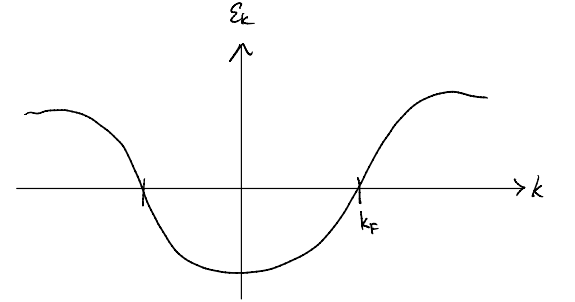
\includegraphics[width=\textwidth]{jupyterbook/data/fig/lec15-fig00.png}
\end{figure}

For a simple dispersion, say a ``consine band'', there is a single Fermi surface defined by $\varepsilon_k=0$. The ground state is then the filled Fermi sea
\[ |\Omega _0\rangle =\prod_{\left| k \right|<\left| k_F \right|}{\hat{c}_{k}^{\dagger}}|0\rangle \]
With this setup we can now evaluate the ``bare propagator''. Remember, the building block of our perturbation theory is the ``basic T-contraction''.
\[ iG_{0}^{F}\left( k,t \right) =\left< \mathcal{T} \left[ \hat{c}_k\left( t \right) \hat{c}_{k}^{\dagger}\left( 0 \right) \right] \right> _0\]
where we have used the fact that our ground state is translation invariant in both space and time (in particular, we used $\left< \hat{c}_k\hat{c}_{k'}^{\dagger} \right> \propto \delta _{kk'}$ to focus on a single momentum). Evaluating
\begin{align*}
    iG_{0}^{F}\left( k,t \right) &=\Theta \left( t \right) \left< \hat{c}_k\left( t \right) \hat{c}_{k}^{\dagger}\left( 0 \right) \right> {\color{red} -}\Theta \left( -t \right) \left< \hat{c}_{k}^{\dagger}\left( 0 \right) \hat{c}_k\left( t \right) \right> \\
    &=\Theta \left( t \right) \Theta \left( \left| k \right|-\left| k_F \right| \right) e^{-i\varepsilon _kt}-\Theta \left( -t \right) \Theta \left( \left| k_F \right|-\left| k \right| \right) e^{-i\varepsilon _kt}
\end{align*}
where the first term is the electron-excitation above the Fermi sea and the second term is the hole-excitation within the Fermi sea. Going to frequency space, we have
\begin{align*}
    iG_{0}^{F}\left( k,\omega \right) &=\int_{-\infty}^{\infty}{dtG_{0}^{F}\left( k,t \right) e^{i\omega t}}\\
    &=\Theta \left( \left| k \right|-\left| k_F \right| \right) \lim_{\eta \rightarrow 0^+} \frac{\left( e^{-\infty}-1 \right)}{i\left( \omega -\varepsilon _k+i\eta \right)}-\Theta \left( \left| k_F \right|-\left| k \right| \right) \lim_{\eta \rightarrow 0^+} \frac{\left( 1-e^{-\infty} \right)}{i\left( \omega -\varepsilon _k-i\eta \right)}
\end{align*}
\[ G_{0}^{F}\left( k,\omega \right) =\lim_{\eta \rightarrow 0^+} \left( \frac{\Theta \left( \left| k \right|-\left| k_F \right| \right)}{\omega -\varepsilon _k+i\eta}+\frac{\Theta \left( \left| k_F \right|-\left| k \right| \right)}{\omega -\varepsilon _k-i\eta} \right) \]
Noticing that the Heaviside step function is simply an ``on-off switch'', it will be natural to further define
\[ \eta _k=\mathrm{sign}\left( \left| k \right|-\left| k_F \right| \right) \eta \]
and we might write
\[ G_{0}^{F}\left( k,\omega \right) =\lim_{\eta _k\rightarrow 0^{\pm}} \frac{1}{\omega -\varepsilon _k+i\eta _k}\]
we call this the (Feynman) propagator.

\begin{figure}[ht]
    \centering
    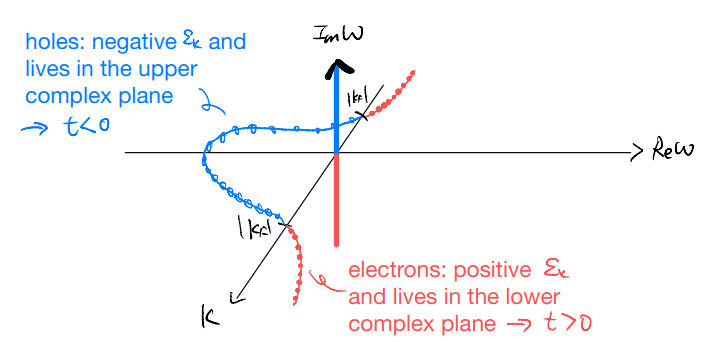
\includegraphics[width=\textwidth]{jupyterbook/data/fig/lec15-fig01.png}
\end{figure}

Notice that, in our single band problem, we have a single pole at each momentum $k$. (Contrast with the phonon propagator, which have two poles for each momentum $k$.) In particular, we see that a single Green's function capture both the electron and hole excitations. The union of the two comes about in an interesting way, with the nature of the excitation (electron versus hole) encoded in the location of the pole (lower versus upper complex plane). In fact, going back to the real-time expression, we see that:
\begin{enumerate}
    \item Electron piece $\Theta \left( t \right) \left< \hat{c}_k\left( 0 \right) \hat{c}_{k}^{\dagger}\left( t \right) \right> $: $t>0$, forward in time
    \item Hole piece $\Theta \left( -t \right) \left< \hat{c}_{k}^{\dagger}\left( 0 \right) \hat{c}_k\left( t \right) \right> $: $t<0$, backward in time
\end{enumerate}

Remarks: The problem of QED electron is completely analogous. The only changes are
\begin{enumerate}
    \item the Fermi ``wave vector'' happens to be $k_F=0$
    \item the ``filled Fermi sea'' is the whole set of negative energy solutions to Dirac equation
    \item we call the ``holes'' positrons
\end{enumerate}
What we mentioned above is a paraphrasing of Feynman's famous interpretation that positron (electron traveling backward in time). (There is a second part of the interpretation: there is only one electron in the universe and it keeps traveling forward and backward. This ``one-electron universe'' is attributed to Wheeler, Feynman's PhD advisor.)

Let us clarify two points before moving on:
\begin{enumerate}
    \item What happened to the spin index? In principle, the one-particle propagator (two-point Green's function) should be a matrix, since each of the two fermions carries an index. (E.g., we simplify the momentum part using $\left< \hat{c}_k\hat{c}_{k'}^{\dagger} \right> \sim \delta _{kk'}$) Correspondingly, when we restore spin indices, we simply have
    \[ G_{\sigma \sigma '}^{F}(k,t)=-i\left< \mathcal{T} \left[ \hat{c}_{k\sigma}\left( t \right) \hat{c}_{k\sigma '}^{\dagger}\left( t \right) \right] \right> \]
    for spin-rotation-invariant system, we also have $\left< \hat{c}_{\sigma}\hat{c}_{\sigma '}^{\dagger} \right> \sim \delta _{\sigma \sigma '}$
    \[ G_{\sigma \sigma '}^{F}\left( k,t \right) =G^F\left( k,t \right) \delta _{\sigma \sigma '}\]
    and so we could focus on the ``single band'' discussion as if the spin did not exist. The spin, however, will actually still be important in giving ``overall factors'' for the different terms in the perturbation expansion.
    \item Some of you might notice that the way we defined the propagator is actually ad hoc in a sense. Let us consider, instead, the contraction
    \begin{align*}
        &\left( -i \right) \left< \mathcal{T} \left[ \hat{c}_{k}^{\dagger}\left( t \right) \hat{c}_k\left( 0 \right) \right] \right> \\
        =&\left( -i \right) \left[ \Theta \left( t \right) \left< \hat{c}_{k}^{\dagger}\left( t \right) \hat{c}_k\left( 0 \right) \right> -\Theta \left( -t \right) \left< \hat{c}_k\left( 0 \right) \hat{c}_{k}^{\dagger}\left( t \right) \right> \right] \\
        =&-ie^{i\varepsilon _kt}\left[ \Theta \left( t \right) \Theta \left( \left| k_F \right|-\left| k \right| \right) -\Theta \left( -t \right) \Theta \left( \left| k \right|-\left| k_F \right| \right) \right] \\
        =&-G_{0}^{F}\left( k,-t \right)
    \end{align*}
    and, as such, we see that this alternative contraction does not provide us with additional data. (But, as a corollary, it also suggest that the ``arrow of time'' we assigned to electrons versus holes is not entirely unambiguous.) Similarly, we may go to frequency space and get
    \[ \left( -i \right) \int_{-\infty}^{\infty}{dt\left< \mathcal{T} \left[ \hat{c}_{k}^{\dagger}\left( t \right) \hat{c}_k\left( 0 \right) \right] \right> e^{i\omega t}}=-\int_{-\infty}^{\infty}{dtG_{0}^{F}\left( k,-t \right) e^{i\omega t}}=-G_{0}^{F}\left( k,-\omega \right) \]
\end{enumerate}

